\section{Comparativo Final --- Visão Completa}

\begin{frame}{Custo por Iteração --- Visão Completa}
    \begin{center}
        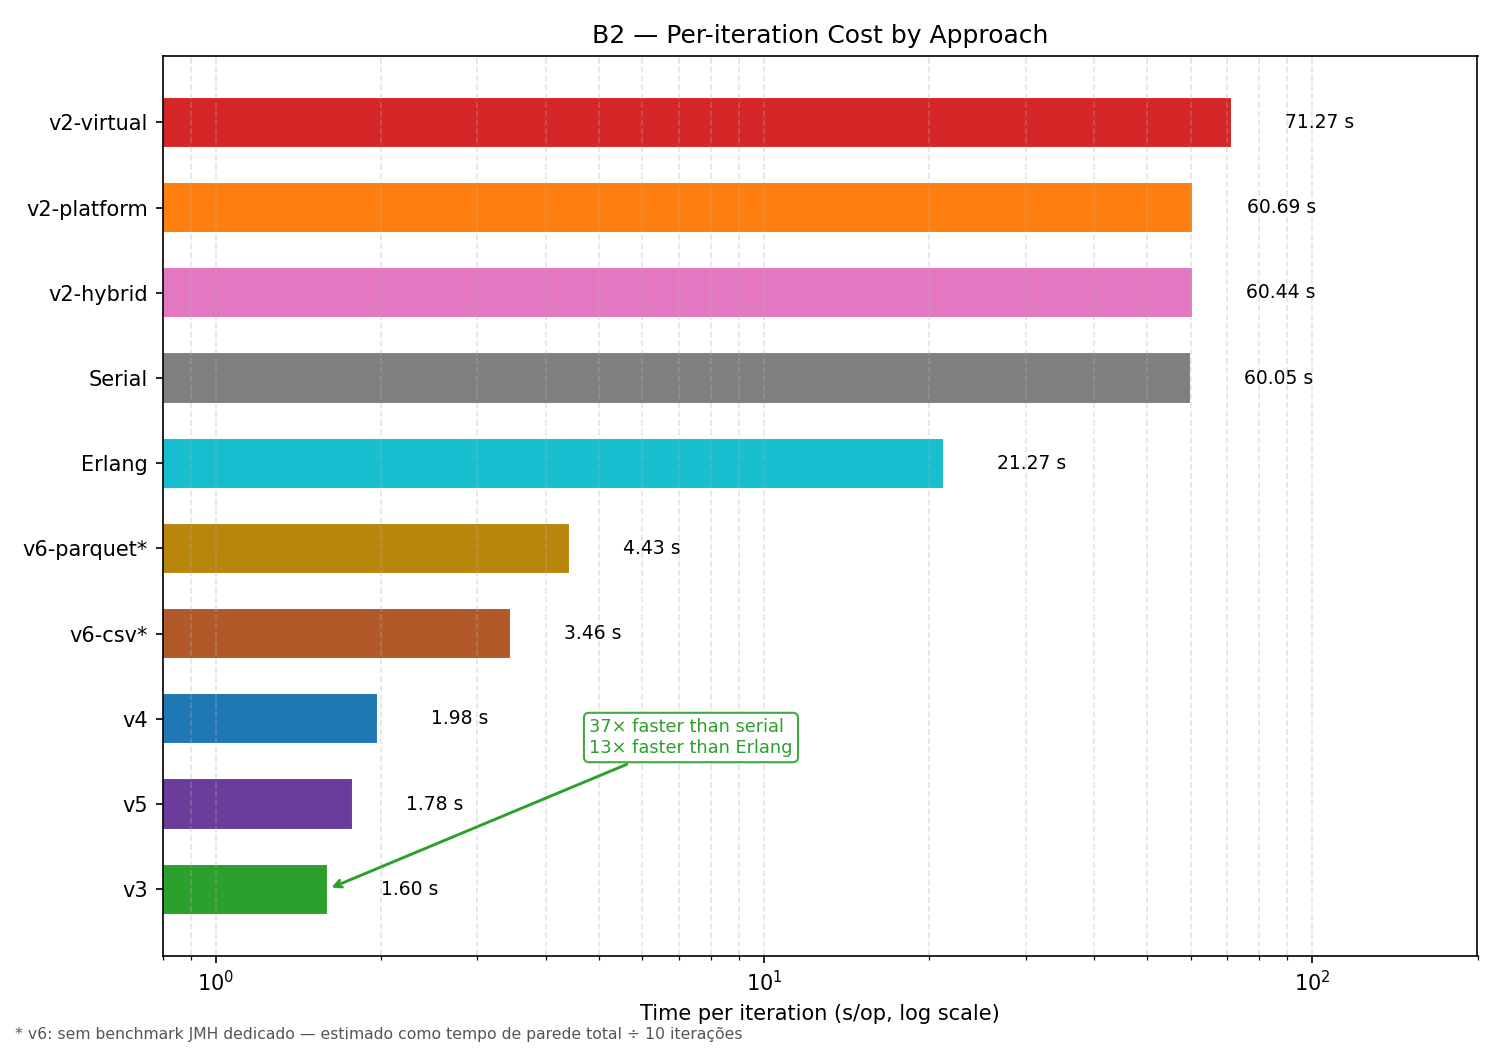
\includegraphics[width=0.85\textwidth]{img/chart1_b2_cost_v4v5v6}
    \end{center}
    {\small v3 segue a mais rápida (1,60 s); v4/v5 ficam perto
    (1,98 / 1,78 s); v6 fica acima de todas ($\approx$3,46 / 4,43 s).}
\end{frame}

\begin{frame}{Evolução do Throughput --- v3, v4 e v5}
    \begin{center}
        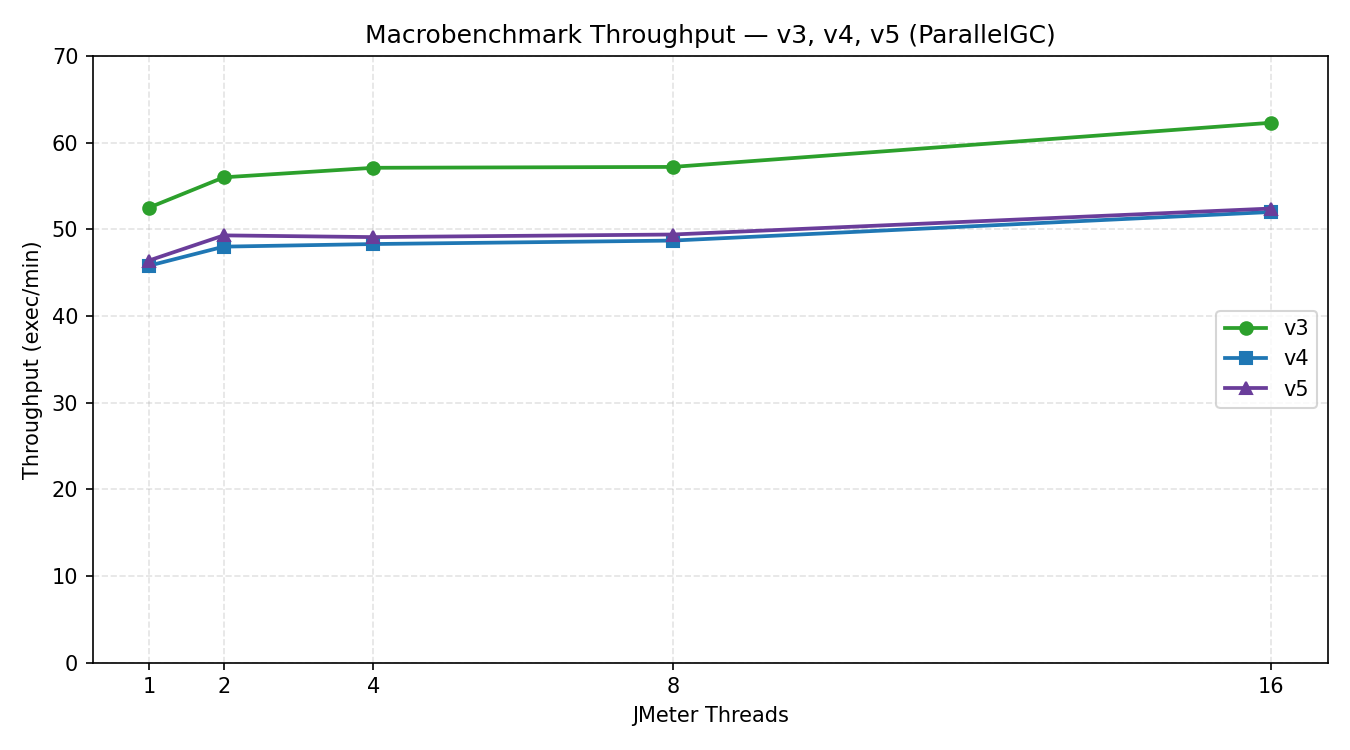
\includegraphics[width=0.85\textwidth]{img/chart5_throughput_v3_v5}
    \end{center}
    {\small Todas com ParallelGC. v6 não aparece --- sem macrobenchmark JMeter
    para o Spark.}
\end{frame}

\begin{frame}{v4 e v5: Robustez e Work-Stealing Têm Custo}
    \begin{itemize}
        \item v4 trocou um bug real (exceção perdida) por
              \alert{$\approx$24\%} de custo extra por iteração
        \item APIs de \textit{preview} ainda não são de graça
        \item v5 não superou a v4 --- \textit{work-stealing} só ajuda com
              carga desbalanceada, e este dataset é uniforme
    \end{itemize}

    \vspace{0.8em}
    \begin{block}{Lição}
        Mudar o idioma de concorrência nem sempre acelera o código.
    \end{block}
\end{frame}

\begin{frame}{Quando Vale a Pena Distribuir}
    \begin{itemize}
        \item Spark (v6) foi mais lento que todas as versões Java nesta
              escala --- o dataset cabe em uma única máquina
        \item Parquet mais lento que CSV: formato de armazenamento também é
              uma variável de desempenho
        \item Cache do Spark falha diferente de uma JVM: degrada aos poucos
              em vez de estourar \texttt{OutOfMemoryError}
    \end{itemize}

    \vspace{0.8em}
    \begin{alertblock}{Conclusão}
        Processamento distribuído compensa quando os dados não cabem mais em
        uma única máquina --- não é o caso aqui.
    \end{alertblock}
\end{frame}
